\subsubsection{\theoryC{High mass dijet resonance search at HE-LHC}}
\contributors{C. Helsens, D. Jamin, M. Selvaggi}
%{\bf Authors: C. Helsens$^1$, D. Jamin$^2$, M. Selvaggi$^3$}\\
%\newline
%$^1$CERN EP-Departement, CH-1211 Geneva 23, Switzerland email: {\tt B.C. clement.helsens@cern.ch}\\
%$^2$Academia Sinica, Institute of  Physics, Taipei, Taiwan\\


%\textbf{Reponsible: Clement Helsens, Michele Selvaggi}

%%%%%%%%%%%%%%%%%%%%%%%%%%%%%%%%%%%%%%%%%%%%%%%%%%%%%%%%%%%%%%%%%%%%%%%%%%%%%%%%%%%%%%%%%%%%
%\subsubsection{Introduction}
\paragraph*{Introduction}
Many models of beyond the SM (BSM) physics predict additional particles with masses at the TeV scale. The presence of new resonant states~\cite{Harris:2011bh,Boelaert:2009jm,Lee:1973iz,Branco:2011iw,Hill:1994hp,Kaplan:1983sm,Bellazzini:2014yua,Randall:1999ee,Pomarol:1999ad} decaying to two highly boosted particles decaying hadronically could be observed as an excess in the QCD dijet distribution. We focus here on the specific benchmark model : excited quark resonance~\cite{Baur:1987ga,Baur:1989kv}. We study the sensitivity in the following decay using hadronic \qjj\ decay mode.

The decay product is typically in the multi-TeV regime and its reconstruction imposes stringent requirement on the detector design. Precise jet energy resolution requires full longitudinal shower containment. High discrimination power and sensitivity for these searches at such extreme energies, requires excellent granularity both in the tracking detectors and calorimeters.

%%%%%%%%%%%%%%%%%%%%%%%%%%%%%%%%%%%%%%%%%%%%%%%%%%%%%%%%%%%%%%%%%%%%%%%%%%%%%%%%%%%%%%%%%%%%
%\subsubsection{Monte Carlo Samples}
\paragraph*{Monte Carlo Samples}
Signal models were generated with {\scshape Pythia}~8.230~\cite{Sjostrand:2014zea} and the LO cross-section is used. The SM background is dijet (QCD), which is generated using {\scshape MG5\_}a{\scshape MC@NLO}~2.5.2~\cite{Alwall:2014hca} at LO. A k-factor of 2 is applied to this background process.

%%%%%%%%%%%%%%%%%%%%%%%%%%%%%%%%%%%%%%%%%%%%%%%%%%%%%%%%%%%%%%%%%%%%%%%%%%%%%%%%%%%%%%%%%%%%
%\subsubsection{Event Selection}
\paragraph*{Event Selection}

Jets are clustered using particle-flow candidates with the anti-$k_T$~\cite{Cacciari:2008gp} algorithm with parameter R=0.4. We require at least two jets with $\pt >1$~TeV and $|\eta|<3$ and the rapidity difference between the two leading jets to be small, $\Delta(\eta)<1.5$ as dijet events will tend to be more central. The dijet invariant mass of the \qjj\ signal for $m_Q^{*}$ and QCD contributions after the full event selection is shown in \fig{fig:hadronicresonances:qqsel01}.

%%%%%%%%%%%%%%%%%%%%%%%%%%%%%%%%%%%%%%%%%%%%%%%%%%%%%%%%%%%%%%%%%%%%%%%%%%%%%%%%%%%%%%%%%%%%
%\subsubsection{Signal extraction and results}
\paragraph*{Signal extraction and results}
Hypothesis testing is performed using a modified frequentist method based on a profile likelihood fit that takes into account the systematic uncertainties as nuisance parameters. The dijet invariant mass is used as a discriminant.

The expected exclusion limit at 95\%~\cl and discovery reach at $5 \sigma$ are shown in middle and right Figures~\ref{fig:hadronicresonances:qqsel01}. The reach for \qjj\ is ~14TeV with \intlumihelhc and it is possible to discover it up to $m_{Q^{*}}=$~12TeV.

\begin{figure}[htbp]
  \centering
  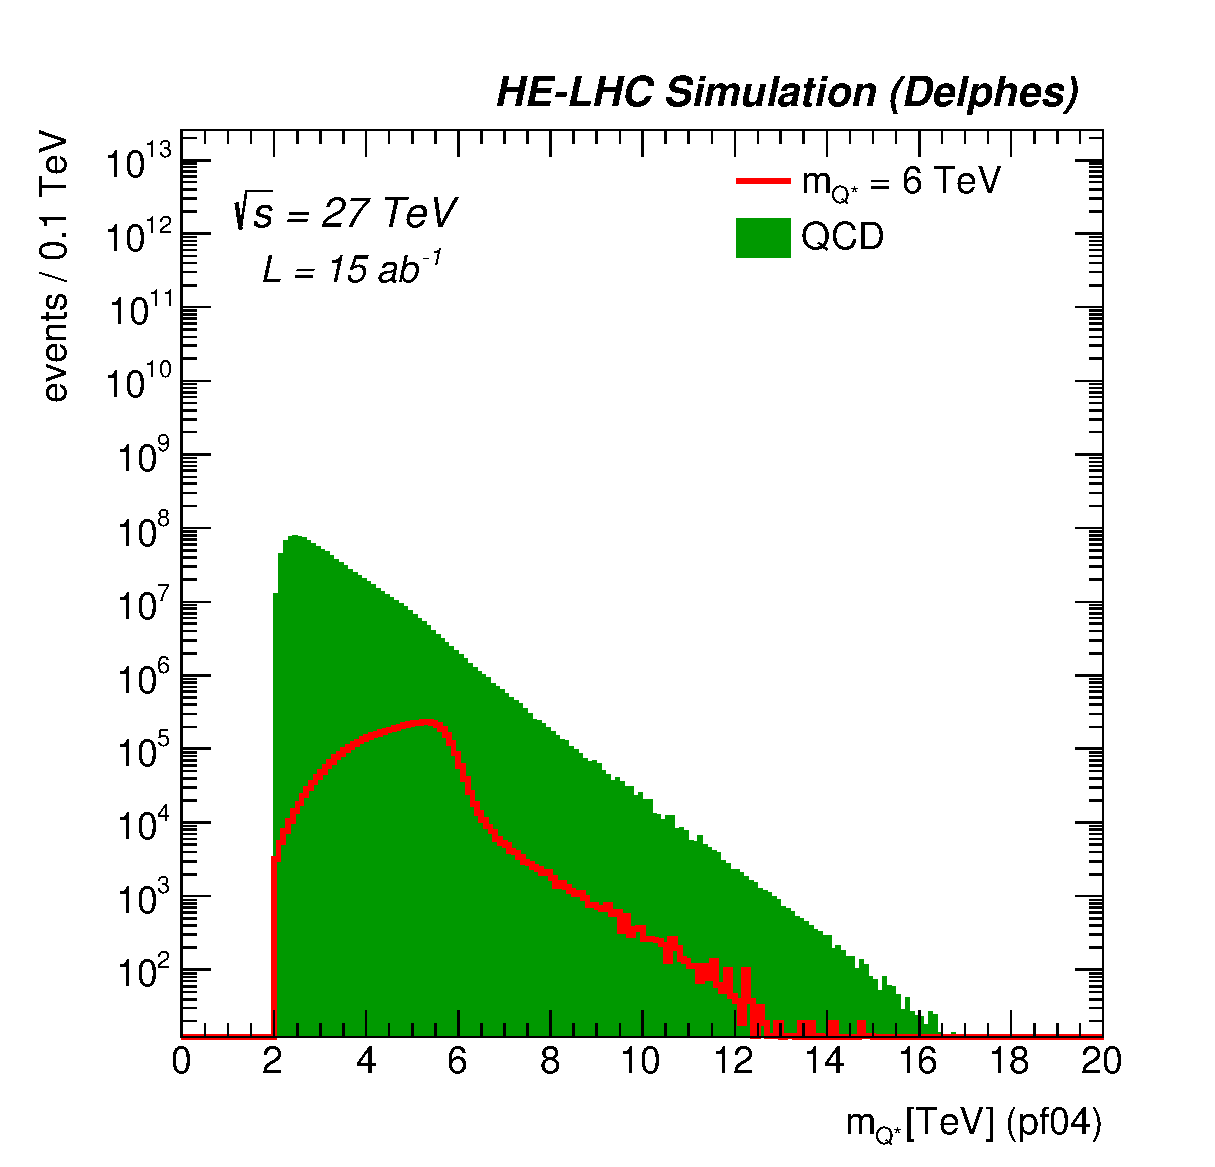
\includegraphics[width=0.30\columnwidth]{\main/section7OtherSignatures/img/qq_Mj1j2_pf04_sel1_nostack_log.eps}
  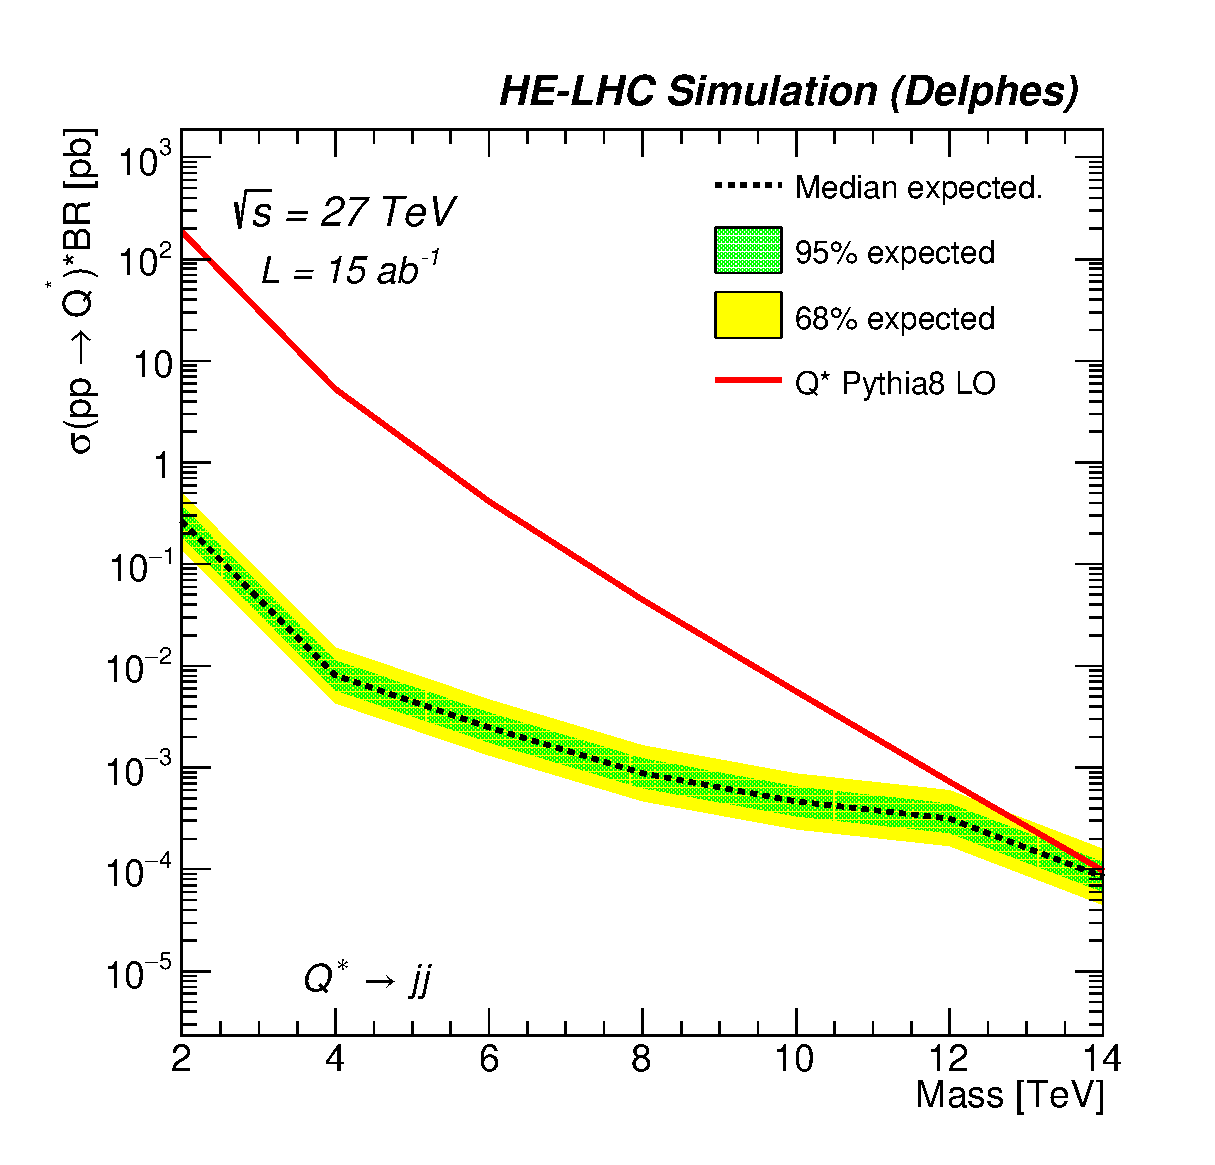
\includegraphics[width=0.30\columnwidth]{\main/section7OtherSignatures/img/lim_Qstar_jj_helhc_v01.eps}
  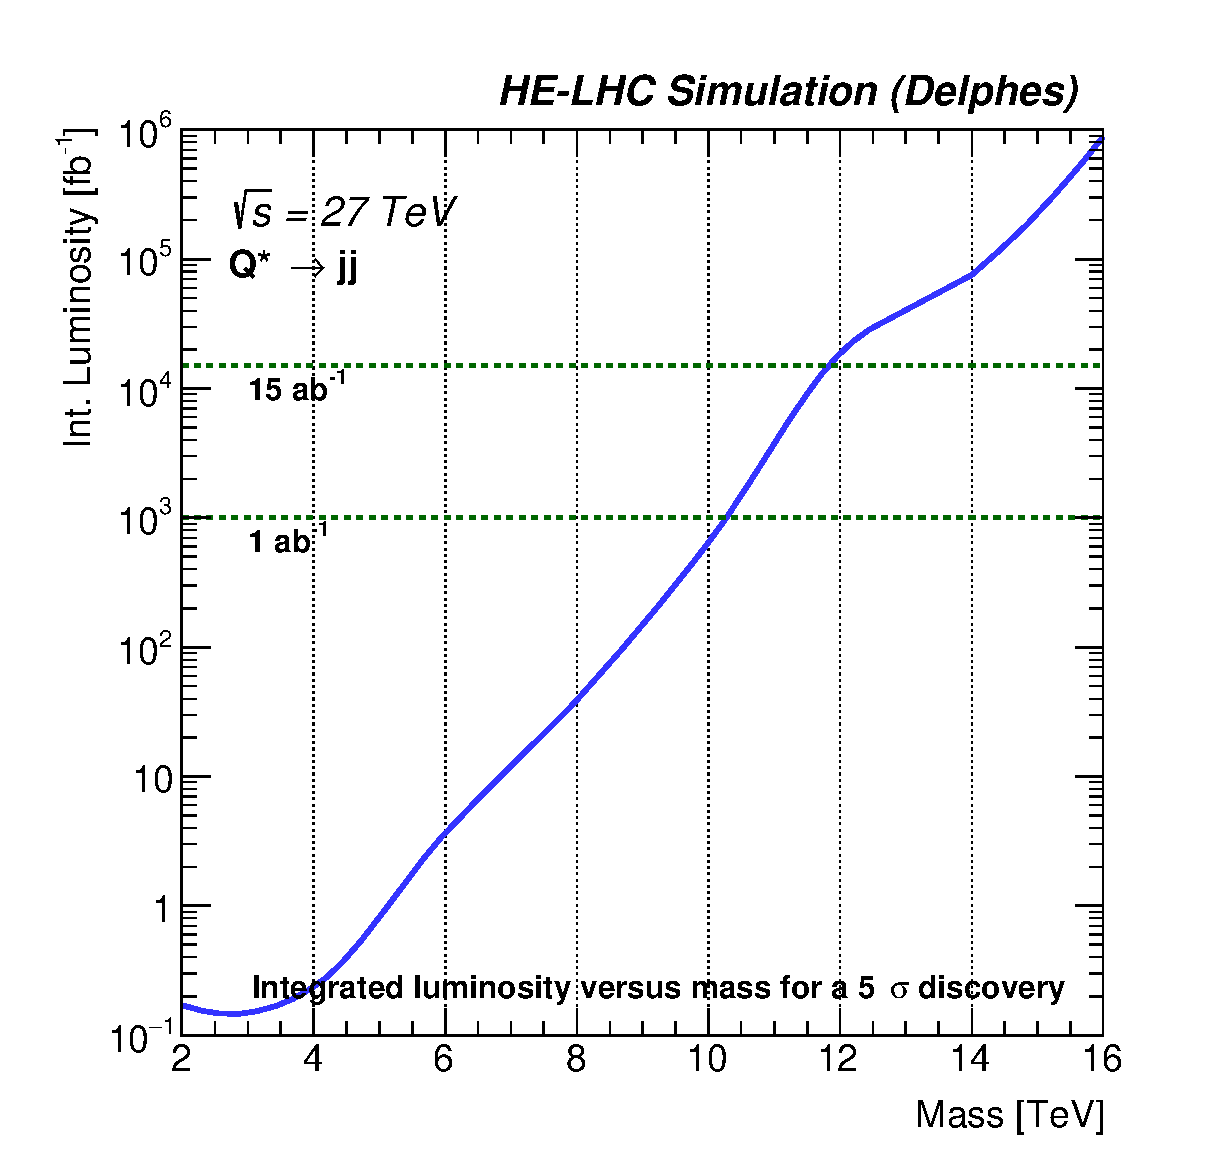
\includegraphics[width=0.30\columnwidth]{\main/section7OtherSignatures/img/DiscoveryPotential_jj_rootStyle.eps}
  \caption{Left distribution : invariant mass distribution of the two leading jets for the full selection for a 6~TeV signal for the \qjj\ analysis. Middle distribution : exclusion limit at 95\%~\cl versus heavy resonance mass. Right distribution : integrated luminosity for a $5\sigma$ discovery as a function of the heavy resonance mass.}
  \label{fig:hadronicresonances:qqsel01}
\end{figure}

\begin{table}[!htb]\centering
\scalebox{0.9}{
\begin{tabular}{|c|c|c|}
\hline
\hline
signal $m_{Z}$  & 2 TeV  &  116820015.2 \\
                & 4 TeV  &   45971584.5 \\
                & 6 TeV  &    5064345.4 \\
                & 8 TeV  &     596530.2 \\
                & 10 TeV &      76228.5 \\
                & 12 TeV &       9978.9 \\
                & 14 TeV &       1314.3 \\
\hline
background      & QCD    & 1144048231.4 \\
\hline
\hline
\end{tabular}}
\caption{Final yield of analysis.}
\label{tab:qqYield}
\end{table}

